	\section{Nombre: Viento multidireccional}\label{obs.vientoM}
	\subsection{Descripción}
		Ráfaga de viento, este objeto no es rígido y puede ser visible solo por las animaciones ocasionales de líneas rectas (horizontales, verticales, diagonales). El viento se activa por lapsos de tiempo constantes. El jugador al entrar en contacto con el viento le estará dando una velocidad constante en una dirección aleatoria que podría ser horizontal, vertical o en diagonal, provocando un "empuje" del personaje. 
	\subsection{Esquema}
	Ver figura \ref{fig:vientoM}.
	\begin{figure}
		\centering
		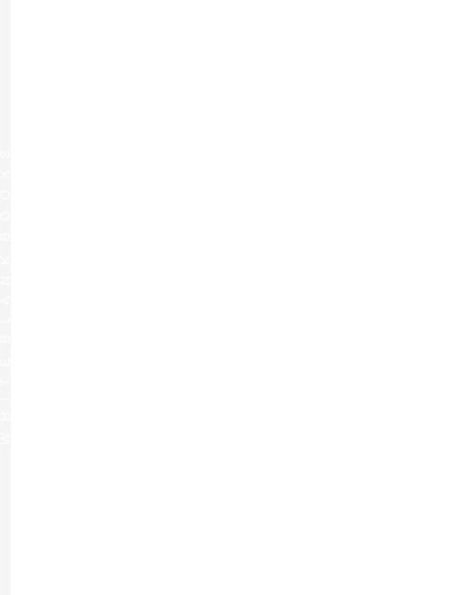
\includegraphics[height=0.2 \textheight]{Imagenes/vientoM}
		\caption{Sacos de cacao.}
		\label{fig:vientoM}
	\end{figure}